\chapter{Reflection}
% Reflect on the course as a whole. Describe what you have learned.Why programming is (or isn’t) important to your future profession? What you liked or didn’t like, how you will apply what you’ve learned in the future and how this course relates to experience design.(300 –500 words)

For starters, I follow two programs, UXD and Technical Informatics, so programming was not new to me. Hence, I did not gain a lot of new programming knowledge from the course. I am familiar with Java, but I have never used processing before. Therefore I did learn a bit about how processing worked.

\medskip

What I did learn during this course was programming from a beginners perspective. Over the years that I've programmed, I learned a lot about how to approach problems in programming. Since it has been some time since I first learned programming, some of these skills have become a second nature, and it has become more difficult for me to imagine not possessing those skills. Seeing my fellow students struggle with the material made me appreciate these skills I've gained. It has also helped me understand how programming can be challenging to someone that has not yet developed these skills yet. In the future, I can use these experiences to better explain programming to none-programmers. I would also be better at communication to non-programmers in a professional setting why certain features might not be as straight forward to implement as they think. 

\medskip

For my career as a programmer, programming is obviously important. My other study mostly focusses on the back-end of programming, with little to no emphasis on creativity. However, I would probably want to become either a full stack developer or front-end developer, as I like to be able to express myself creatively while programming. A course like this is perfect in that regard, since it is more design oriented and creative expression through programming is its goal. 

\medskip

The importance of programming to UXD can in my opinion be summarized in the Venn diagram shown in \cref{fig: venn diagram}.

\begin{figure}[H]
    \centering
    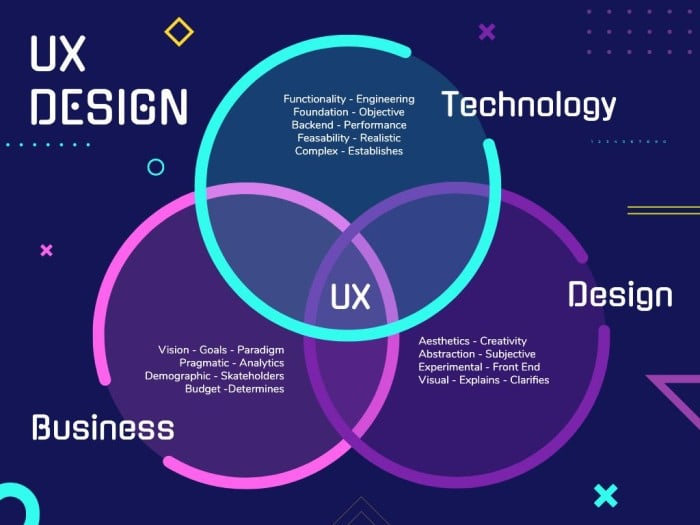
\includegraphics[width = 0.55\textwidth]{Figures/reflection/venn_diagram.jpg}
    \caption{Diagram relating technology, business and design together}
    \label{fig: venn diagram}
\end{figure}

In the figure, UXD is shown to be the combination of design business and technology. Design was the main topic of design \& creativity and Introduction to UX. Business was the main topic of Professional Skills and Research for Design. Technology was not really covered so far and I think this course is the first time this facet of UX was touched upon. 